\documentclass[a4paper,10pt,fleqn]{article}
\usepackage{fullpage}
\setlength{\mathindent}{0pt}

% do not indent first line of paragraph.
\setlength{\parindent}{0cm}
% But separate them with 3-10mm
\setlength{\parskip}{6mm plus4mm minus3mm}

\usepackage[dutch]{babel}
\usepackage[utf8]{inputenc}

\usepackage{amsmath}
\usepackage{amssymb}
%~ \usepackage{tabularx}

% Hyperref package, clickable internal links.
% colorlinks to remove ugly boxes around links...
% \usepackage[colorlinks]{hyperref}

\makeatletter
\newcommand*{\centerfloat}{%
  \parindent \z@
  \leftskip \z@ \@plus 1fil \@minus \textwidth
  \rightskip\leftskip
  \parfillskip \z@skip}
\makeatother

\usepackage{enumerate}

\usepackage{subfigure}
\usepackage{pgf}
\usepackage{tikz}
\usetikzlibrary{arrows,automata, shapes}

\title{TI2736-A Assignment 2:  Bayesan network}

\author{
    David Akkerman - 4220390 \\
    Jan Pieter Waagmeester - 1222848 \\
}

\begin{document}
\maketitle

\section*{2.1: A simple network I}
\begin{enumerate}[1.]
    % Compute the chance that the customer wants to purchase fruit (i.e., ‘P (F )’). Please write down an exact equation for P (F ) before filling it in. This will help you a lot for the later questions.
    \item $$P(F) = \sum_{\forall i} \sum_{\forall j} (P(F|V_iH_j) \cdot P(V_i) \cdot P(H_j)) = 0.29$$

    % 2. Compute the chance that the customer wants to purchase candy. Again, start with the exact equation for P (C ).
    \item $$P(C) = \sum_{\forall i} \sum_{\forall j} (P(C|H_iK_j) \cdot P(H_i) \cdot P(K_j)) = 0.42 $$

    % Now assume that our customer is a vegetarian: “evidence is found that our customer is a vegetarian”.

    % 3. Compute the chance that this customer wants to purchase fruit.
    \item $$P(F|V) = \sum_{\forall i} P(F|VH_i) \cdot P(H_i) = 0.79 $$

    % 4. And what is the chance that the vegetarian customer wants to purchase candy?
    \item $$P(C|V) = P(C) = 0.42$$

    % 5. Does the fact that the customer is a vegetarian change our belief in the customer having healthy eating habits? I.e., does P (H ) change, now that we known that V is true?
    % Please give your answer using a maximum of 30 words.
    \item Nee, voor de berekeningen is aangenomen dat $V$ en $H$ onafhankelijk zijn. Dit betekent dus dat geldt: $$P(H|V) = P(H)$$ Dit betekent dat $P(H)$ niet verandert als $V$ bekend is.

    % 6. What is the chance that this customer wants to purchase fruit?
    \item $$P(F|V\lnot H) = 0.7$$

    % 7. And what is the chance for this customer to purchase candy?
    \item $$P(C|V\lnot H) = P(C|\lnot H) = \sum_{\forall i} P(C|\lnot HK_i) \cdot P(K_i) = 0.58     $$

    % 8. What is the chance that this customer wants to purchase fruit?
    \item $$P(F|\lnot V, H, \lnot K) = P(F|\lnot V,H) = 0.9 $$

    % 9. And what is the chance for this customer to purchase candy?
    \item $$P(C|\lnot V, H, \lnot K) = P(C|H,\lnot K) = 0.01    $$

\end{enumerate}

\section*{2.2: A simple network II}

\begin{enumerate}[1.]
    \setcounter{enumi}{9}

    % 10. In the lecture you have seen Bayes’ rule, e.g. in the “cold” example. Use Bayes’ rule to derive an expression for P(V |M). Express your answer using only known odds (Eqs.2.1 - 2.11, Eqs. 2.12 - 2.13). If done correctly, your equation should be of the form P(V |M) = a/a+b
    \item
        \begin{align*}
            P(V|M)
                & = \frac{P(M|V)\cdot P(V)}{P(M)} \\
                & = \frac{P(M|V)\cdot P(V)}{P(M|V)\cdot P(V) + P(M|\lnot V)\cdot P(\lnot V)} \\
                & = 4.4 \cdot 10^{-5} \\
            P(M)
                & = \sum_{\forall i} P(M|V_i) \cdot (V_i) = 0.91 \\
        \end{align*}

    % 11. Compute the chance that the customer is a vegetarian, given that he does not want to purchase any meat (P(V |¬M)).
    \item
        \begin{align*}
            P(V|\lnot M)
                & = \frac{P(\lnot M|V) \cdot P(V)}{P(\lnot M)} \\
                & = 0.44
        \end{align*}

    % 12. A similar, but yet more complicated, equation may be written down to compute P(V |F). The only real difference is the fact that you will need an extra elimination of variables.
    \item
        % ziet er een beetje lelijk uit in code, maar nu past het binnen de pagina
        \begin{align*}
            P(V|F)
                & = \frac{P(F|V)\cdot P(V)}{P(F)}  \\
                & = \frac{
                        P(F|VH) \cdot P(V) \cdot P(H) +
                        P(F|V \lnot H) \cdot P(V) \cdot P(\lnot H)
                      }{
                        \left( \parbox{10cm}{
                            $$P(F|VH) \cdot P(V) \cdot P(H) +
                            P(F|V \lnot H) \cdot P(V) \cdot P(\lnot H) +$$
                            $$P(F|\lnot VH) \cdot P(\lnot V) \cdot P(H) +
                            P(F|\lnot V\lnot H) \cdot P(\lnot V) \cdot P(\lnot H)$$
                        } \right)
                      }
        \end{align*}

    % 13. Compute the chance that the customer is a vegetarian, given that he does want to purchase fruit (P (V |F )).
    \item
        \begin{align*}
            P(V| F) & = 0,11 \\
        \end{align*}

    % 14. Now, write down an equation for P (V |M F ). If done correctly, your equation should be of the form P (V |M F ) = (a+c)/(a+c+b+d)

    \item
        \begin{align*}
            P(V |M, F)
                & = \frac{P(M,F|V)\cdot P(V)}{P(M,F)} \\
                & = \frac{P(M|V)\cdot P(F|V)\cdot P(V)}{P(M)\cdot P(F)} \\
                & = \frac{P(M|V)\cdot P(V)\cdot P(F|VH)\cdot P(H) + P(M|V)\cdot P(V)\cdot P(V\lnot H)\cdot P(\lnot H)}{P(M|V)\cdot P(V)\cdot P(F|VH)\cdot P(H) + P(M|V)\cdot P(V)\cdot P(V\lnot H)\cdot P(\lnot H) + }
        \end{align*}

    % 15. Compute the chance that the customer is a vegetarian, given that he does want to purchase fruit, but no meat (P (V |F ¬M )).
    \item
        \begin{align*}
            P(V |F, \neg M) & = \\
        \end{align*}


\end{enumerate}

\section*{2.3: A non-boolean network}
\begin{enumerate}[1.]
    \setcounter{enumi}{15}
    % 16. Write down an equation for P (H ) using the terms listed in Eqs. 2.14 - 2.18.
    \item
        \begin{align*}
            P(H) &= P(H|S_1) \cdot P(S_1) + P(H|S_2) \cdot P(S_2) + P(H|S_3) \cdot  P(S_3) \\
        \end{align*}

    % 17. Compute P (H ) and P (¬H ).
    \item De kans op $S_3$ is niet gegeven, maar kan worden berekend:


        \begin{align*}
          P(S_3)    & = (1 - 0.05 - 0.35)\\
                    & = 0.6 \\
          \intertext{Daarna is $P(H)$ eenvoudig:}
          P(H)      & = 0.2 \cdot 0.05 + 0.5 \cdot 0.35 + 0.9 \cdot P(S_3) \\
                    & = 0.665 \\
          P(\neg H) & = 1 - P(H)\\
                    & = 0.335 \\
        \end{align*}

    % 18. Use the knowledge acquired in As. 2.2 to compute the chance that the customer is an inactive sporter, given that the customer has healthy eating habbits.
    \item
        \begin{align*}
            P(S_1 | H)  & = \frac{P(H|S_1) \cdot P(S_1)}{P(H)} \\
                        & = \frac{0.2 \cdot 0.05}{0.335} \\
                        & = 0.015\\
        \end{align*}


\end{enumerate}

\section*{2.4: A network for our robot}
\begin{enumerate}[1.]
    \setcounter{enumi}{19}
    % 19. Give a schematic diagram of the network relevant to the above text. Show all the proper variables and causalities. (Hint: There are 5 variables in total)
    \item Een schematische weergave van dit netwerk:

    \tikzstyle{every node}=[
            draw, ellipse, minimum width=1.5cm, minimum height=1cm, align=center]
    \begin{centering}

        \begin{tikzpicture}[node distance=3cm, auto, bend angle=45]
            \node (M) {M};
            \node (H) [right of=M] {H};
            \node (E2) [below left of=M] {2, Flowers};
            \node (E1) [right of=E2] {1, Junk food};
            \node (E3) [right of=E1] {3, Salads};

            \path[-latex]
                (M) edge (E2)
                    edge (E1)
                (H) edge (E1)
                    edge (E3);
        \end{tikzpicture}
    \end{centering}

    % 20. write down all the conditional- and a-priori probabilities.
    \item
        A-priori-kansen:
        \begin{align*}
            P(M)                    & = 0.84 \\
            P(H)                    & = 0.30 \\
        \intertext{Conditionele kansen:}
            P(1 | H, M)             & = 0.86 \\
            P(1 | H, \neg M)        & = 0.57 \\
            P(1 | \neg H, M)        & = 0.56 \\
            P(1 | \neg H, \neg M)   & = 0.90 \\
            P(2 | M)                & = 0.34 \\
            P(2 | \neg M)           & = 0.64 \\
            P(3 | H)                & = 0.88 \\
            P(3 | \neg H)           & = 0.64 \\
        \end{align*}


    % 21. Expand the network with the given probabilities. Make a diagram of the nodes with arrows indicating the direction of influence (H = Healthy, M = Married, C = Children, V = Vegetarian, F = Female).
     \item Hier de afbeelding uitgebreid met de gegeven kansen.

    \begin{centering}
        \begin{tikzpicture}[node distance=2.6cm, auto,scale=0.5]

            \node (M) {\textbf{M}arried};
            \node (H) [right of=M] {\textbf{H}ealthy};
            \node (C) [right of=H] {\textbf{C}hildren};
            \node (V) [right of=C] {\textbf{V}egetarian};
            \node (F) [right of=V] {\textbf{F}emale};

            \begin{scope}[node distance=2cm]
              \node (E2) at (-2, -6) {2};
              \node (E1) [right of=E2] {1};
              \node (E3) [right of=E1] {3};
              \node (E6) [right of=E3] {6};
              \node (E5) [right of=E6] {5};
              \node (E4) [right of=E5] {4};
              \node (E7) [right of=E4] {7};
             \end{scope}

            \path[-latex]
                (M) edge (E2)
                    edge (E1)
                (H) edge (E1)
                    edge (E3)
                    edge (E5)
                (C) edge (E3)
                    edge (E4)
                    edge (E6)
                (V) edge (E3)
                    edge (E5)
                (F) edge (E4)
                    edge (E7);
        \end{tikzpicture}
    \end{centering}

    % 22. Make a screenshot of your network for in the report.
    \item In GeNIe ziet het er dan als volgt uit:
        \begin{figure}[!ht]
        \centering
        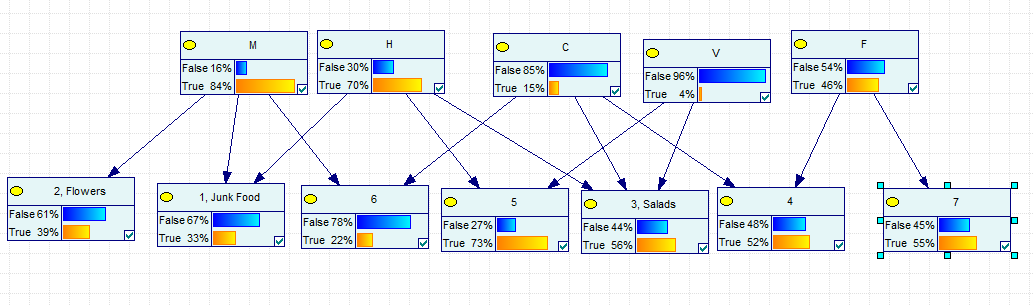
\includegraphics[width=1\textwidth]{images/genie}
    \end{figure}

    % 23. What’s the probability the customer will want to buy products from class 5?
    \item $73\%$

    % 24. What’s the probability the customer will not want anything from class 2?
    \item $39\%$

    % 25. Given that the customer is a female. What is the probability of having to buy something in class 4?
    \item $71\%$

    % 26. This same woman turns out to have two children. What is the chance of her wanting something from class 4 now?
    \item $86\%$, ook direct afleesbaar uit tabel.

    % 27. A different customer profiles as a healthy vegetarian. What’s the probability of buying a product from class 3?
    \item $95\%$

    % 28. A customer was seen buying something out of class 2. What is the probability that he/she is married?
    \item $74\%$

    % 29. What’s the chance this customer is female?
    \item Deze kans is niet afhankelijk van van categorie 2, $46\%$

    % 30. A wealthy man was observed to buy products from all categories. What is the probability that he’s is married?
    \item $24\%$

    % 31. Another customer appeared to not buy anything from the listed classes. What can you say about this customer?
    \item Zeer waarschijnlijk is deze persoon getrouwd, maar niet gezond, en geen vrouw. Deze persoon heeft vrijwel zeker geen kinderen en is geen vegetarier.

    % 32. We know that a certain person bought stuff from class 1 and 2, but we did not observe the rest of his basket. Is this person likely to have any children?
    \item Waarschijnlijk niet, de kans is slechts $15\%$.

    % 33. We do not know what a given person bought, but we are certain he didn’t buy anything from class 2, 3 or 5. What can you say about this customer?
    \item We weten niet zeker of het een man of een vrouw is, maar deze persoon is vrijwel zeker getrouwd, maar niet gezond en heeft waarschijnlijk geen kinderen. De kans dat deze persoon vegetarier is is erg klein.
\end{enumerate}

\end{document}
